\iffalse
\title{ME:2014}
\author{AI24BTECH11007}
\section{me}
\chapter{2014}
\fi
                              
	\item
		Consider a two-dimensional laminar flow over a long cylinder as shown in figure below.\\
		\vspace{0.5cm}
            \begin{center}
		    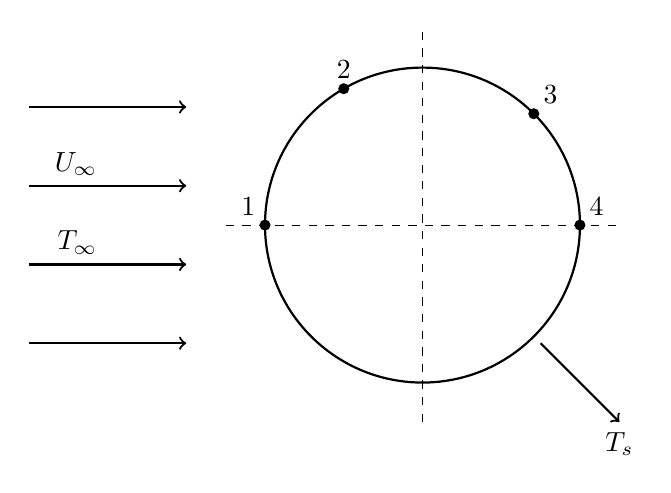
\begin{tikzpicture}
    % Draw the circle
    \draw[thick] (0,0) circle(2);

    % Draw the dots on the circle with labels
    \fill (2,0) circle(2pt) node[above right] {4};
    \fill (-2,0) circle(2pt) node[above left] {1};
    \fill (-1,1.732) circle(2pt) node[above] {2};
    \fill (1.414,1.414) circle(2pt) node[above right] {3};

    % Draw center dashed lines
    \draw[dashed] (-2.5,0) -- (2.5,0); % Horizontal
    \draw[dashed] (0,-2.5) -- (0,2.5); % Vertical

    % Draw the arrow with T_s label
    \draw[->, thick] (1.5,-1.5) -- (2.5,-2.5) node[below] {$T_s$};

    % Draw flow lines on the left side with labels
    \draw[->, thick] (-5, 1.5) -- (-3, 1.5);
    \draw[->, thick] (-5, 0.5) -- (-3, 0.5) node[midway, above left] {$U_\infty$};
    \draw[->, thick] (-5, -0.5) -- (-3, -0.5) node[midway, above left] {$T_\infty$};
    \draw[->, thick] (-5, -1.5) -- (-3, -1.5);
\end{tikzpicture}

	    \end{center}
		\vspace{0.5cm}
		The free stream velocity is $U_{\infty}$ and the free stream temperature $T_{\infty}$ is lower than the cylinder surface temperature $T_s$. The local heat transfer coefficient is minimum at a point 

		\hfill{(ME:2014)}
    \begin{multicols}{4}
    \begin{enumerate}
        \item $1$
        \item $2$
        \item $3$
        \item $4$
    \end{enumerate}
    \end{multicols}

\vspace{0.5cm}

    \item For a completely submerged body with centre of gravity $G$ and centre of buoyancy $B$, the condition of stability will be: 

	   	    
	    \hfill{(ME:2014)}
    \begin{multicols}{2}
    \begin{enumerate}
        \item $G$ is located below $B$
        \item $G$ is located above $B$
        \item $G$ and $B$ are coincident
        \item Independent of the locations of $G$ and $B$
    \end{enumerate}
    \end{multicols}
\vspace{0.5cm}
    \item In a power plant, water (density $= 1000 \, {kg/m}^3$) is pumped from $80 \, kPa$ to $3 \, MPa$. The pump has an isentropic efficiency of $0.85$. Assuming that the temperature of the water remains the same, the specific work (in $kJ/kg$) supplied to the pump is: 
	    
	    \hfill{(ME:2014)}
    \begin{multicols}{4}
    \begin{enumerate}
        \item $0.34$
        \item $2.48$
        \item $2.92$
        \item $3.43$
    \end{enumerate}
    \end{multicols}

    \item Which one of the following is a CFC refrigerant?
	   
	    \hfill{(ME:2014)}
    \begin{multicols}{4}
    \begin{enumerate}
        \item $R744$
        \item $R290$
        \item $R502$
        \item $R718$
    \end{enumerate}
    \end{multicols}
\vspace{0.5cm}
    \item The jobs arrive at a facility, for service, in a random manner. The probability distribution of the number of arrivals of jobs in a fixed time interval is: 

	    \hfill{(ME:2014)}
		\begin{multicols}{4}
    \begin{enumerate}
        \item Normal
        \item Poisson
        \item Erlang
        \item Beta
    \end{enumerate}
    \end{multicols}
\vspace{0.5cm}
    \item In exponential smoothing method, which one of the following is true? 
	    \hfill{(ME:2014)}
    \begin{enumerate}
        \item $0 \leq \alpha \leq 1$ and high value of $\alpha$ is used for stable demand
        \item $0 \leq \alpha \leq 1$ and high value of $\alpha$ is used for unstable demand
        \item $\alpha \geq 1$ and high value of $\alpha$ is used for stable demand
        \item $\alpha \leq 0$ and high value of $\alpha$ is used for unstable demand
    \end{enumerate}
\vspace{0.5cm}
    \item For machining a rectangular island represented by coordinates $P(0,0)$, $Q(100,0)$, $R(100,50)$, and $S(0,50)$ on a casting using CNC milling machine, an end mill with a diameter of $16 \, mm$ is used. The trajectory of the cutter center to machine the island $PQRS$ is:

	    \hfill{(ME:2014)}
    \begin{enumerate}
        \item $(-8, -8), (108, -8), (108, 58), (-8, 58), (-8, -8)$
        \item $(8,8), (94,8), (94,44), (8,44), (8,8)$
        \item $(-8,8), (94,0), (94,44), (8,44), (-8,8)$
        \item $(0,0), (100,0), (100,50), (50,0), (0,0)$
    \end{enumerate}
\vspace{0.5cm}
    \item Which one of the following instruments is widely used to check and calibrate geometric features of machine tools during their assembly? 
	    \hfill{(ME:2014)}
    \begin{multicols}{2}
    \begin{enumerate}
        \item Ultrasonic probe
        \item Coordinate Measuring Machine (CMM)
        \item Laser interferometer
        \item Vernier calipers
    \end{enumerate}
    \end{multicols}

    \item The major difficulty during welding of aluminium is due to its: 

	    \hfill{(ME:2014)}
    \begin{multicols}{2}
    \begin{enumerate}
        \item High tendency of oxidation
        \item High thermal conductivity
        \item Low melting point
        \item Low density
    \end{enumerate}
    \end{multicols}

    \item The main cutting force acting on a tool during the turning (orthogonal cutting) operation of a metal is $400 \, N$. The turning was performed using $2 \, mm$ depth of cut and $0.1 \, mm/rev$ feed rate. The specific cutting pressure (in N/mm$^2$) is:

	    \hfill{(ME:2014)}
    \begin{multicols}{4}
    \begin{enumerate}
        \item $1000$
        \item $2000$
        \item $3000$
        \item $4000$
    \end{enumerate}
    \end{multicols}

    \item
	    The process of reheating the martensitic steel to reduce its brittleness without any significant loss in its hardness is: 

	    \hfill{(ME:2014)}
    \begin{multicols}{4}
    \begin{enumerate}
        \item Normalising
        \item Annealing
        \item Quenching
        \item Tempering
    \end{enumerate}
    \end{multicols}

    \item In solid-state welding, the contamination layers between the surfaces to be welded are removed by:

	    \hfill{(ME:2014)}
    \begin{multicols}{4}
    \begin{enumerate}
        \item Alcohol
        \item Plastic deformation
        \item Water jet
        \item Sand blasting
    \end{enumerate}
    \end{multicols}

    \item The integral $\oint_C (y \, dx - x \, dy)$ is evaluated along the circle $x^2 + y^2 = \frac{1}{4}$ traversed in counterclockwise direction. The integral is equal to: 

	    \hfill{(ME:2014)}
    \begin{multicols}{4}
    \begin{enumerate}
        \item $0$
	\item $-\frac{\pi}{4}$
	\item $\frac{ \pi}{4}$
	\item $-\frac{ \pi}{2}$
    \end{enumerate}
    \end{multicols}


